\documentclass{article}\usepackage[]{graphicx}\usepackage[]{color}
%% maxwidth is the original width if it is less than linewidth
%% otherwise use linewidth (to make sure the graphics do not exceed the margin)
\makeatletter
\def\maxwidth{ %
  \ifdim\Gin@nat@width>\linewidth
    \linewidth
  \else
    \Gin@nat@width
  \fi
}
\makeatother

\definecolor{fgcolor}{rgb}{0.345, 0.345, 0.345}
\newcommand{\hlnum}[1]{\textcolor[rgb]{0.686,0.059,0.569}{#1}}%
\newcommand{\hlstr}[1]{\textcolor[rgb]{0.192,0.494,0.8}{#1}}%
\newcommand{\hlcom}[1]{\textcolor[rgb]{0.678,0.584,0.686}{\textit{#1}}}%
\newcommand{\hlopt}[1]{\textcolor[rgb]{0,0,0}{#1}}%
\newcommand{\hlstd}[1]{\textcolor[rgb]{0.345,0.345,0.345}{#1}}%
\newcommand{\hlkwa}[1]{\textcolor[rgb]{0.161,0.373,0.58}{\textbf{#1}}}%
\newcommand{\hlkwb}[1]{\textcolor[rgb]{0.69,0.353,0.396}{#1}}%
\newcommand{\hlkwc}[1]{\textcolor[rgb]{0.333,0.667,0.333}{#1}}%
\newcommand{\hlkwd}[1]{\textcolor[rgb]{0.737,0.353,0.396}{\textbf{#1}}}%
\let\hlipl\hlkwb

\usepackage{framed}
\makeatletter
\newenvironment{kframe}{%
 \def\at@end@of@kframe{}%
 \ifinner\ifhmode%
  \def\at@end@of@kframe{\end{minipage}}%
  \begin{minipage}{\columnwidth}%
 \fi\fi%
 \def\FrameCommand##1{\hskip\@totalleftmargin \hskip-\fboxsep
 \colorbox{shadecolor}{##1}\hskip-\fboxsep
     % There is no \\@totalrightmargin, so:
     \hskip-\linewidth \hskip-\@totalleftmargin \hskip\columnwidth}%
 \MakeFramed {\advance\hsize-\width
   \@totalleftmargin\z@ \linewidth\hsize
   \@setminipage}}%
 {\par\unskip\endMakeFramed%
 \at@end@of@kframe}
\makeatother

\definecolor{shadecolor}{rgb}{.97, .97, .97}
\definecolor{messagecolor}{rgb}{0, 0, 0}
\definecolor{warningcolor}{rgb}{1, 0, 1}
\definecolor{errorcolor}{rgb}{1, 0, 0}
\newenvironment{knitrout}{}{} % an empty environment to be redefined in TeX

\usepackage{alltt}

\usepackage{amsmath}
\IfFileExists{upquote.sty}{\usepackage{upquote}}{}
\begin{document}


        
\begin{enumerate}
        
\item %1

\begin{enumerate}
\item

Type II Sums of Squares were used.



\begin{center}
\begin{tabular}{|c|c|}
\hline \hline
SSE & \ensuremath{6.2505657\times 10^{7}}\\
MSE & \ensuremath{4.1670438\times 10^{6}}\\
$SS_{trt}$ & \ensuremath{1.0319149\times 10^{8}}\\
$MS_{trt}$ & \ensuremath{2.5797872\times 10^{7}}\\
F-stat & 6.190929\\
p-value & 0.003786\\
\hline
\end{tabular}
\end{center}

\item %1b

Let i and j index the 1-5 voltage levels.

$H_{0}$: $\mu_{i} = \mu_{j}$ for all i $\neq$ j

$H_{A}$: at least one $\mu_{i} \neq \mu_{j}$ for all i $\neq$ j

\item %1c

Below are the five sample variances.
% latex table generated in R 3.3.2 by xtable 1.8-2 package
% Sun Jan 29 20:21:58 2017
\begin{table}[ht]
\centering
\begin{tabular}{||l|l||}
  \hline
  \hline
$s^{2}_{1}$ & 1329.58 \\ 
  $s^{2}_{2}$ & 62.92 \\ 
  $s^{2}_{3}$ & 4846188.25 \\ 
  $s^{2}_{4}$ & 15987486.00 \\ 
  $s^{2}_{5}$ & 152.25 \\ 
   \hline
\end{tabular}
\end{table}


\item %1d

Below are diagnostic plots.

\begin{knitrout}
\definecolor{shadecolor}{rgb}{0.969, 0.969, 0.969}\color{fgcolor}
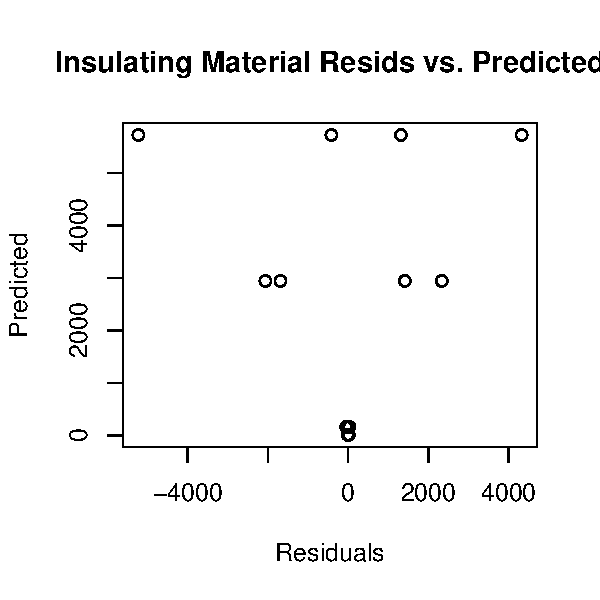
\includegraphics[width=\maxwidth]{figure/prob1d-1} 

\end{knitrout}

\begin{knitrout}
\definecolor{shadecolor}{rgb}{0.969, 0.969, 0.969}\color{fgcolor}
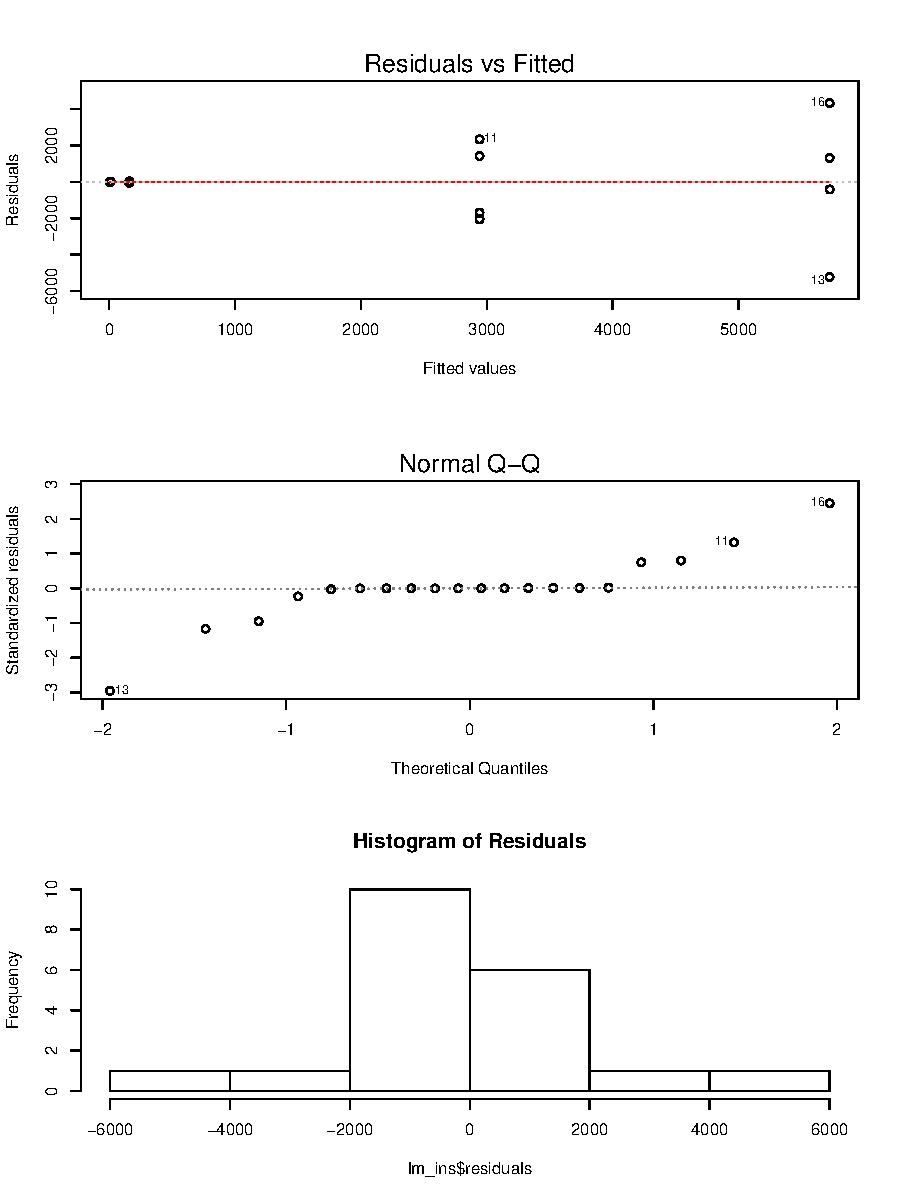
\includegraphics[width=\maxwidth]{figure/prob1dx-1} 

\end{knitrout}

The constant variance assumption is the most concerning violation, but the normal Q-Q plot also shows the tails of residuals are more extreme than would be expected under normality. Without correcting for the non-constant variance, the p-value from the F-test will be too small because there is extra variation we aren't accounting for, making us more likely to find evidence of significant differences that do not exist.

\item %1e
The constant variance assumption violation is the most concerning, and without any more work, I would most likely not report these results. If I {\it were} to make a conclusion, it would be there is strong evidence the mean failure time differs between at least two voltage levels.
\end{enumerate}

\item %2

\begin{enumerate}
\item %2a
Assume $\tau_{2}$ = 0.



X = $\begin{bmatrix}
 1 & 1 & 0\\
 1 & 1 & 0\\
 1 & 1 & 0\\
 1 & 1 & 0\\
 1 & 0 & 0\\
 1 & 0 & 0\\
 1 & 0 & 0\\
 1 & 0 & 0\\
 1 & 0 & 1\\
 1 & 0 & 1\\
 1 & 0 & 1\\
 1 & 0 & 1\\
 \end{bmatrix}$
 
 $X^{T}X$ = $\begin{bmatrix}
 12 & 4 & 4\\
 4 & 4 & 0\\
 4 & 0 & 4\\
 \end{bmatrix}$
 
 $(X^{T}X)^{-1}$ = $\begin{bmatrix}
 0.25 & -0.25 & -0.25\\
 -0.25 & 0.5 & 0.25\\
 -0.25 & 0.25 & 0.5
 \end{bmatrix}$
 
 {\bf fix this -- somethings wrong tapply(df$y,as.factor(df$x),mean)}
 
 $X^{T}Y$ = $\begin{bmatrix}
 445\\
 119\\
 179
 \end{bmatrix}$
 

\item %2b

$\theta = \begin{bmatrix}
\mu \\
\theta_{dosage=20}\\
\theta_{dosage=40}
\end{bmatrix}$

$\mu$ = the true mean observation for dosage 20

$\theta_{dosage = 30}$ = the true change in mean observational units between the mean for dosage 20 and the mean for dosage 30

$\theta_{dosage = 40}$ = the true change in mean observational units between the mean for dosage 20 and the mean for dosage 40


\item %2c

$\hat{\theta} = \begin{bmatrix} 36.75\\
-7\\
8
\end{bmatrix}$

\item %2d
{\it Assume} $\Sigma \tau_{i}$ = 0.



Let $\tau_{3} = \tau_{1} + \tau_{2}$

X = $\begin{bmatrix}
 1 & 1 & 0\\
 1 & 1 & 0\\
 1 & 1 & 0\\
 1 & 1 & 0\\
 1 & 0 & 1\\
 1 & 0 & 1\\
 1 & 0 & 1\\
 1 & 0 & 1\\
 1 & -1 & -1\\
 1 & -1 & -1\\
 1 & -1 & -1\\
 1 & -1 & -1\\
 \end{bmatrix}$
 
 $X^{T}X$ = $\begin{bmatrix}
 12 & 0 & 0\\
 0 & 8 & 4\\
 0 & 4 & 8\\
 \end{bmatrix}$
 
 $(X^{T}X)^{-1}$ = $\begin{bmatrix}
 0.083 & 0 & 0\\
 0 & 0.167 & -0.083\\
 0 & -0.83 & 0.167
 \end{bmatrix}$
 
 $X^{T}Y$ = $\begin{bmatrix}
 445\\
 -60\\
 -32
 \end{bmatrix}$
 
\item

$\theta = \begin{bmatrix}
\mu\\
\theta_{dosage=30}\\
\theta_{dosage=40}
\end{bmatrix}$

$\mu$ = the true mean observation over all dosages

$\theta_{dosage = 30}$ = the true change in mean observational units between the overall mean and the mean for dosage 30

$\theta_{dosage = 40}$ = the true change in mean observational units between the overall mean and the mean for dosage 40

\item %2f

$\hat{\theta}$ = $\begin{bmatrix}
37.0833333\\

-7.3333333\\

-0.3333333
\end{bmatrix}$


\end{enumerate}

Remaining problems are attached.

\end{enumerate}
\end{document}
